Dieses Kapitel  behandelt in Kurzform  die wichtigsten Grundlagen,  welche zum
Verst\"andnis des Versuches erforderlich sind. Die detaillierten Herleitungen
sind in der Versuchsanleitung zu finden~\cite{ref:looser:skineffekt}.

% **************************************************************************** %
\subsection{Grundidee}
\label{sec:arbgru:subsec:grundidee}
% **************************************************************************** %

Hochfrequente  Wechselstr\"ome  haben  die   Eigenschaft,  dass  sie  v.a.  an
der  Oberfl\"ache  eines  Leiters  fliessen  und  nicht  tief  in  den  Leiter
eindringen. Dieses als  \emph{Skineffekt} bekannte  Ph\"anomen soll  in diesem
Versuch experimentell nachgewiesen werden.

Wird  ein  Leiter  in  ein  wechselndes  Magnetfeld  eingef\"uhrt,  werden  in
ihm  Wirbelstr\"ome  induziert. Ist  die  Frequenz  des  externen  Magnetfelds
niedrig,  verteilen  sich  diese  Wirbelstr\"ome  (ungleichm\"assig)  auf  den
gesamten  Querschnitt.  Bei  h\"oheren  Frequenzen  des externen  Magnetfeldes
verlagern   sich   die   Wirbelstr\"ome  in   den   Oberfl\"achenbereich   des
Leiters. Da sie  der \"Anderung  des externen  Feldes gem\"ass  der Lenz'schen
Regel~\cite{ref:wikipedia:lenzscheRegel}  entgegenwirken,  schw\"achen sie  im
Innern  des  Leiters  das  externe  Feld  ab. Ebenfalls  werden  der  Ohm'sche
Widerstand und der Selbstinduktionskoeffizient der Konfiguration von Spule und
Zylinder ge\"andert, sowie der magnetische Fluss im Innern des Zylinders.

Als Versuchsf\"alle dienen die  F\"alle eines eingef\"uhrten Hohlzylinders und
eines  eingef\"uhrten Vollzylinders. Es werden  sowohl g\"angige  N\"aherungen
wie  auch die  exakten  L\"osungen  aus der  Theorie  mit den  Messergebnissen
verglichen.


% **************************************************************************** %
\subsection{Vollzylinder}
\label{sec:arbgru:subsec:vollzylinder}
% **************************************************************************** %

\begin{figure}[th!]
    \centering
    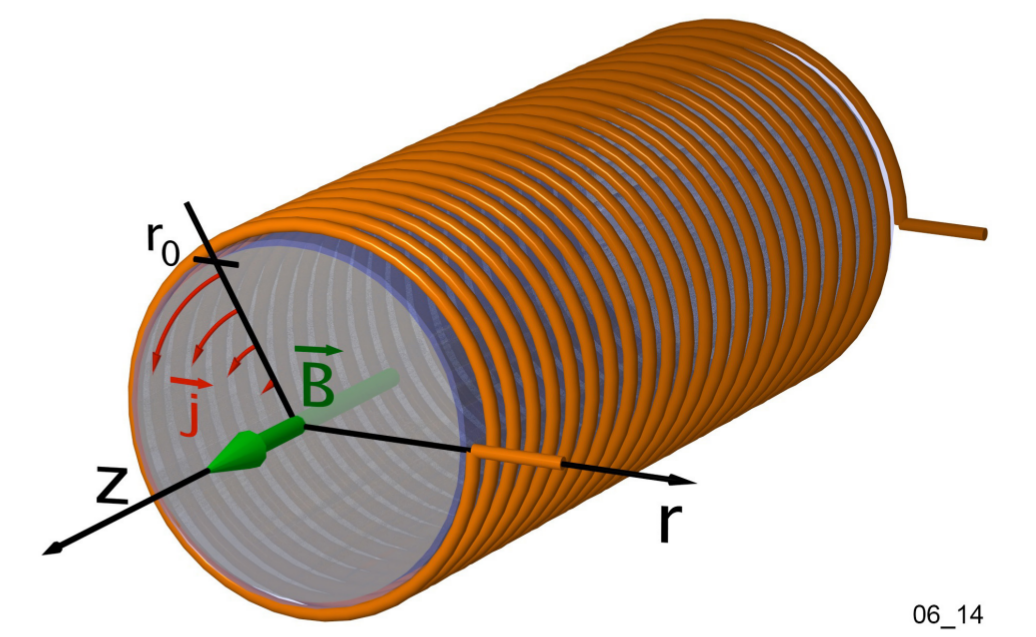
\includegraphics[width=.5\textwidth]{images/spule-vollzylinder.png}
    \caption{Spule mit Vollzylinder \emph{Quelle:} Skript zum Versuch~\cite{ref:looser:skineffekt}}
\end{figure}


% ---------------------------------------------------------------------------- %
\subsubsection{B-Feld, exakte L\"osung}
\label{sec:arbgru:subsec:vollzylinder:bFeldexakt}
% ---------------------------------------------------------------------------- %


Die exakte Beschreibung des Magnetfelds innerhalb des Leiters ist die L\"osung der
folgenden Differentialgleichung:

\begin{equation}
    \label{eq:vollzylinder:DLG}
        0 = r^2 \cdot \hat{B}'' (r) + r\ \cdot \hat{B}' (r) - i \cdot \omega\mu_0\sigma \cdot r^2 \cdot \hat{B} (r) \\
\end{equation}

wobei:

\begin{itemize}
    \item[]
        $r$: Distanz zu Zylinderachse
    \item[]
        $\hat{B}$: gemessenes Magnetfeld im Innern des Leiters (komplexe Gr\"osse)
    \item[]
        $\omega$: Kreisfrequenz des \"ausseren Magnetfeldes
    \item[]
        $\sigma$: spezifische Leitf\"ahigkeit des eingef\"uhrten Leiters
\end{itemize}


Die L\"osung dieser Differentialgleichung (g\"ultig f\"ur beliebige Frequenzen und Positionen) ist:
\begin{equation}
    \label{eq:vollzylinder:bFeldExact}
    \hat{B} (r) = \frac{J_0 (k \cdot r)}{J_0 (k \cdot r_0)} \cdot \hat{B}_0,
\end{equation}

wobei
\begin{itemize}
    \item[]
        $k = \sqrt{\frac{\omega \cdot \mu_0 \cdot \sigma}{2}} \cdot (1-i)$
    \item[]
        $r_0$: Radius des eingef\"uhrten Zylinders
    \item[]
        $\hat{B}_0$: \"Ausseres Magnetfeld (erzeugt von Zylinderspule)
    \item[]
        $J_0(z)$: Besselfunktion erster Art (siehe auch~\cite{ref:wikipedia:bessel})
\end{itemize}

\emph{Beachte}: $\hat{B} (r)$ ist eine komplexe Zahl!


% ---------------------------------------------------------------------------- %
\subsubsection{B-Feld, Hochfrequenzn\"aherung}
\label{sec:arbgru:subsec:vollzylinder:bFeldapprox}
% ---------------------------------------------------------------------------- %


Im Falle hoher Frequenzen kann man folgende N\"aherung verwenden:

\begin{equation}
    \label{eq:vollzylinder:bFeldApprox}
    \hat{B} (x) = \hat{B}_0 \cdot exp\Biggl(-\frac{x}{s_{skin}} \Biggr) \cdot exp\Biggl(-i \cdot \frac{x}{s_{skin}} \Biggr)
\end{equation}

wobei
\begin{itemize}
    \item[]
        $s_{skin} = \sqrt{\frac{2}{\omega \cdot \mu_0 \cdot \sigma}}$
    \item[]
        Die L\"osung brauchbar ist f\"ur $s_{skin} << r_0$.
\end{itemize}




% ---------------------------------------------------------------------------- %
\subsubsection{Selbstinduktionskoeffizient und Ohm'scher Widerstand, exakte L\"osung}
\label{sec:arbgru:subsec:vollzylinder:LRexakt}
% ---------------------------------------------------------------------------- %

Der Selbstinduktionskoeffizient der Konfiguration aus Spule und Leiter ergibt:
\begin{equation}
    \label{eq:vollzylinder:LExact}
    L = \frac{\mu_0 \cdot 2\pi \cdot r_0 \cdot N_0^2}{l} \cdot Re \Biggl(\frac{J_1 (k \cdot r_0)}{k \cdot J_0 (k \cdot r_0)} \Biggr) + L_{Rand}
\end{equation}

wobei
\begin{itemize}
    \item[]
        $l$: L\"ange der Zylinderspule
    \item[]
        $N_0$: Anzahl Windungen der Zylinderspule
    \item[]
        $L_{Rand} = \frac{\mu_0 \cdot 2\pi \cdot r_0 \cdot (r_{Sp} - r_0) \cdot N_0^2}{l}$ mit $r_{Sp}$: Radius Zylinderspule
\end{itemize}

Der Ohm'sche Widerstand errechnet sich zu:
\begin{equation}
    \label{eq:vollzylinder:RExact}
    R_{\Omega,tot} = - \frac{\mu_0 \cdot 2\pi \cdot r_0 \cdot N_0^2}{l} \cdot Im \Biggl(\frac{J_1 (k \cdot r_0)}{k \cdot J_0 (k \cdot r_0)} \Biggr) + R_{\Omega,0}
\end{equation}

Wobei $R_{\Omega,0}$ der  Ohm'sche Widerstand der Zylinderspule  ist (also des
Drahts, aus dem die Spule konstruiert ist).

Letztlich noch der auf den Spulenstrom normierten magnetischen Fluss:

\begin{equation}
    \label{eq:vollzylinder:phiExact}
    \frac{\hat{\Phi}}{\hat{I}} = \frac{\mu_0 \cdot 2\pi \cdot r_0 \cdot N_0^2}{l} \cdot \Biggl(\frac{J_1 (k \cdot r_0)}{k \cdot J_0 (k \cdot r_0)} + r_{Sp} - r_0 \Biggr)
\end{equation}


% **************************************************************************** %
\subsection{Hohlzylinder}
\label{sec:arbgru:subsec:hohlzyliner}
% **************************************************************************** %


\begin{minipage}[c][][b]{0.475\textwidth}
    \centering
    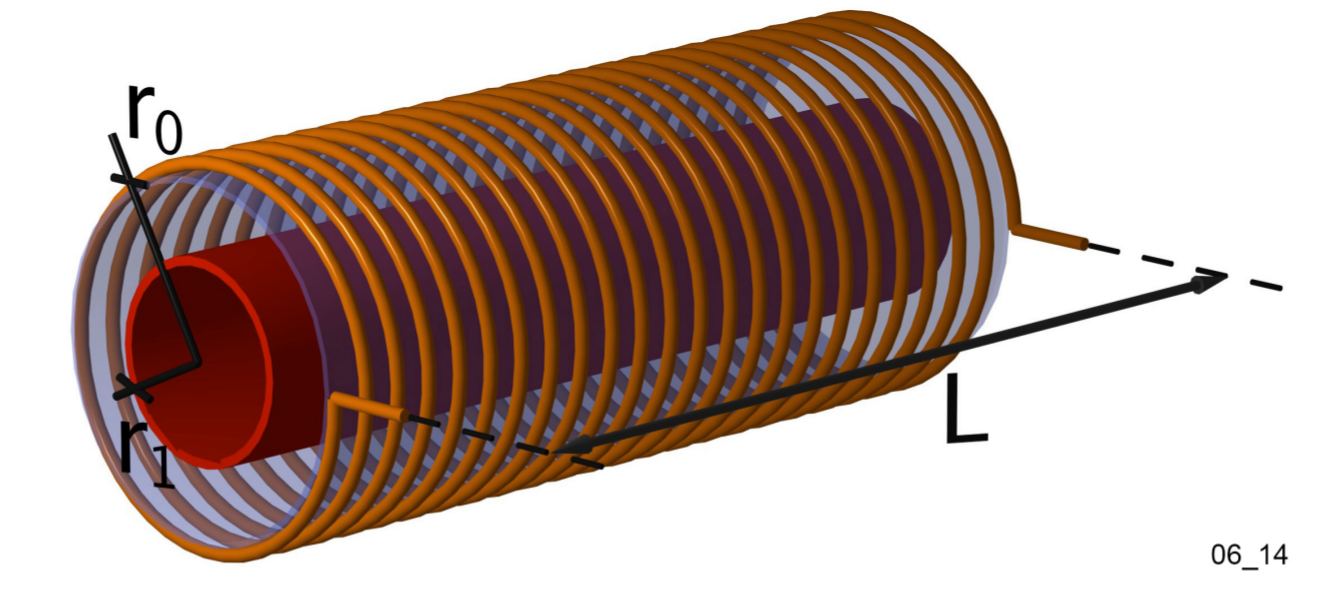
\includegraphics[width=.8\textwidth]{images/spule-hohlzylinder.png}
    \captionof{figure}{Spule mit Hohlzylinder \emph{Quelle:} Skript zum Versuch~\cite{ref:looser:skineffekt}}
\end{minipage}
\begin{minipage}[c][][b]{0.475\textwidth}
    \centering
    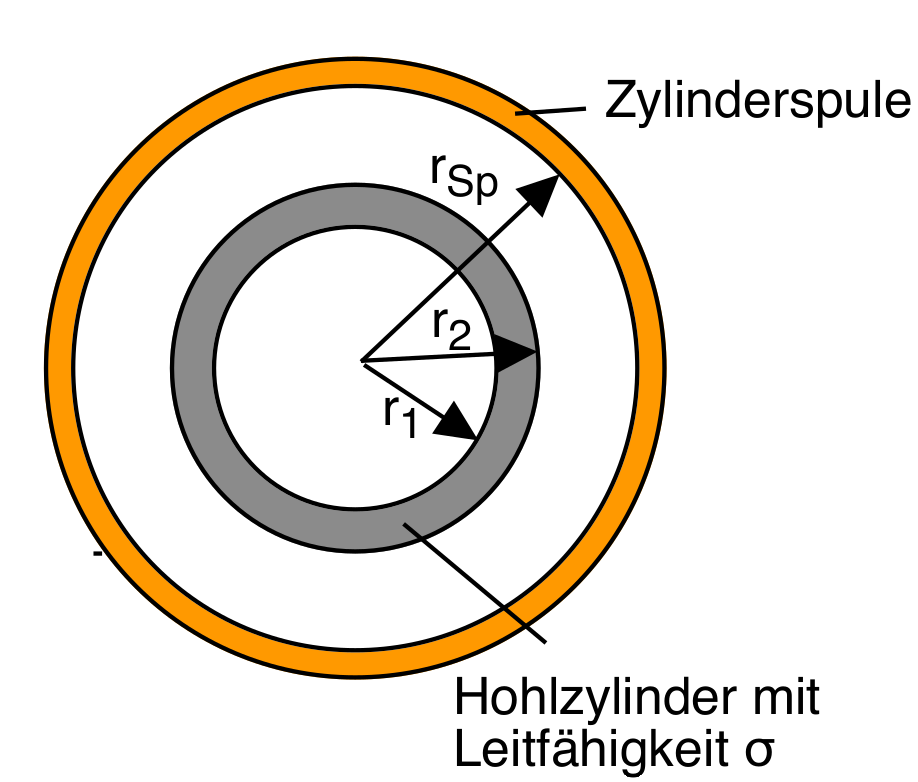
\includegraphics[width=.8\textwidth]{images/spule-hohlzylinder-querschnitt.png}
    \captionof{figure}{Spule mit Hohlzylinder, Querschnitt \emph{Quelle:} Skript zum Versuch~\cite{ref:looser:skineffekt}}
\end{minipage}


% ---------------------------------------------------------------------------- %
\subsubsection{B-Feld, exakte L\"osung}
\label{sec:arbgru:subsec:hohlzylinder:BExact}
% ---------------------------------------------------------------------------- %

\begin{align}
    \label{eq:hohlzylinder:BExact}
    0 \leq r \leq r_1:      \hat{B} (r) & = \hat{B} (r_1) = konst. \\
    r_1 \leq r \leq r_2:    \hat{B} (r) & = \frac{J_{0,r} \cdot Y_{2,r_1} - J_{2,r_1} \cdot Y_{0,r}}{J_{0,r_2} \cdot Y_{2,r_1} - J_{2,r_1} \cdot Y_{0,r_2}} \cdot \hat{B}_0 \\
    r_2 \leq r \leq r_{Sp}: \hat{B} (r) & = \hat{B}_0 = konst.
\end{align}

Mit $J_{0,r_i} = J_0 (k \cdot r_i)$ und $k$ gem\"ass Abschnitt zum Vollzylinder.

% ---------------------------------------------------------------------------- %
\subsubsection{B-Feld, N\"aherungsl\"osung niedrige Frequenzen}
\label{sec:arbgru:subsec:hohlzylinder:BApprox}
% ---------------------------------------------------------------------------- %

Solange die  Wandst\"arke kleiner ist  als die Eindringtiefe  $s_{skin}$, kann
das Rohr als d\"unnwanding betrachtet und folgende Formel verwendet werden:
\begin{equation}
    \label{eq:hohlzylinder:BApprox}
    B_{tot} = \frac{\mu_0 \cdot N_0 \cdot I_0}{l} \cdot \Biggl( \frac{2}{i \cdot \omega \cdot \mu_0 \cdot r_1 \cdot d \cdot \sigma + 2} \Biggr)
\end{equation}


wobei:

\begin{itemize}
    \item[]
        $r_1$: mittlerer Radius des Metallrohrs
    \item[]
        $d$: Wandst\"arke des Metallrohrs
\end{itemize}

% ---------------------------------------------------------------------------- %
\subsubsection{Selbstinduktionskoeffizient und Ohm'scher Widerstand, exakte L\"osung}
\label{sec:arbgru:subsec:hohlzylinder:LRexakt}
% ---------------------------------------------------------------------------- %


\begin{align}
    \label{eq:hohlzylinder:phiNormExact}
    \begin{split}
    \frac{\hat{\Phi}}{\hat{I}} & = \frac{\mu_0 \cdot N_0^2}{l} \\
                               & \cdot \Biggl( r_1^2 \cdot \frac{J_{0,r_1} \cdot Y_{2,r_1} - J_{2,r_1} \cdot Y_{0,r_1}}{J_{0,r_2} \cdot Y_{2,r_1} - J_{2,r_1} \cdot Y_{0,r_2}} \\
                               & + \frac{2}{k} \frac{r_2 \cdot (J_{1,r_2} \cdot Y_{2,r_1} - J_{2,r_1} \cdot Y_{1,r_2}) - r_1 \cdot (J_{1,r_1} \cdot Y_{2,r_1} - J_{2,r_1} \cdot Y_{1,r_1})}{J_{0,r_2} \cdot Y_{2,r_1} - J_{2,r_1} \cdot Y_{0,r_2}} \\
                               & + (r_{Sp}^2 - r_2^2) \Biggr)
    \end{split} \\
    L & = Re \Biggl(\frac{\hat{\Phi}}{\hat{I}} \Biggr) \\
    R & = - \omega \cdot Im \Biggl(\frac{\hat{\Phi}}{\hat{I}} \Biggr) + R_{\Omega,0}
\end{align}
